\subsubsection{Decision Trees and Random Forests}
	Another popular type of classifiers stems from the concept of decision trees (\cite{quinlan2014c4}). That is, a flow chart consisting of decision intersections (called nodes) flows from a starting root (the tree stem). The data is further segmented in each following junction until a state is achieved, in which ideally all segments are "pure", containing observation belonging to a single class. Note that Decision Trees and other Ensemble Methods are not well suited for classification of \hyperref[data_sparsity]{sparse data}, due to the large number of features. This means the information gain from each note is very minor. A segment of a Decision Tree implemented in sparse data is graphically illustrated in Figure \ref{fig:rand_forest_sparse}.
	
	\begin{figure}[h]
		\centering
		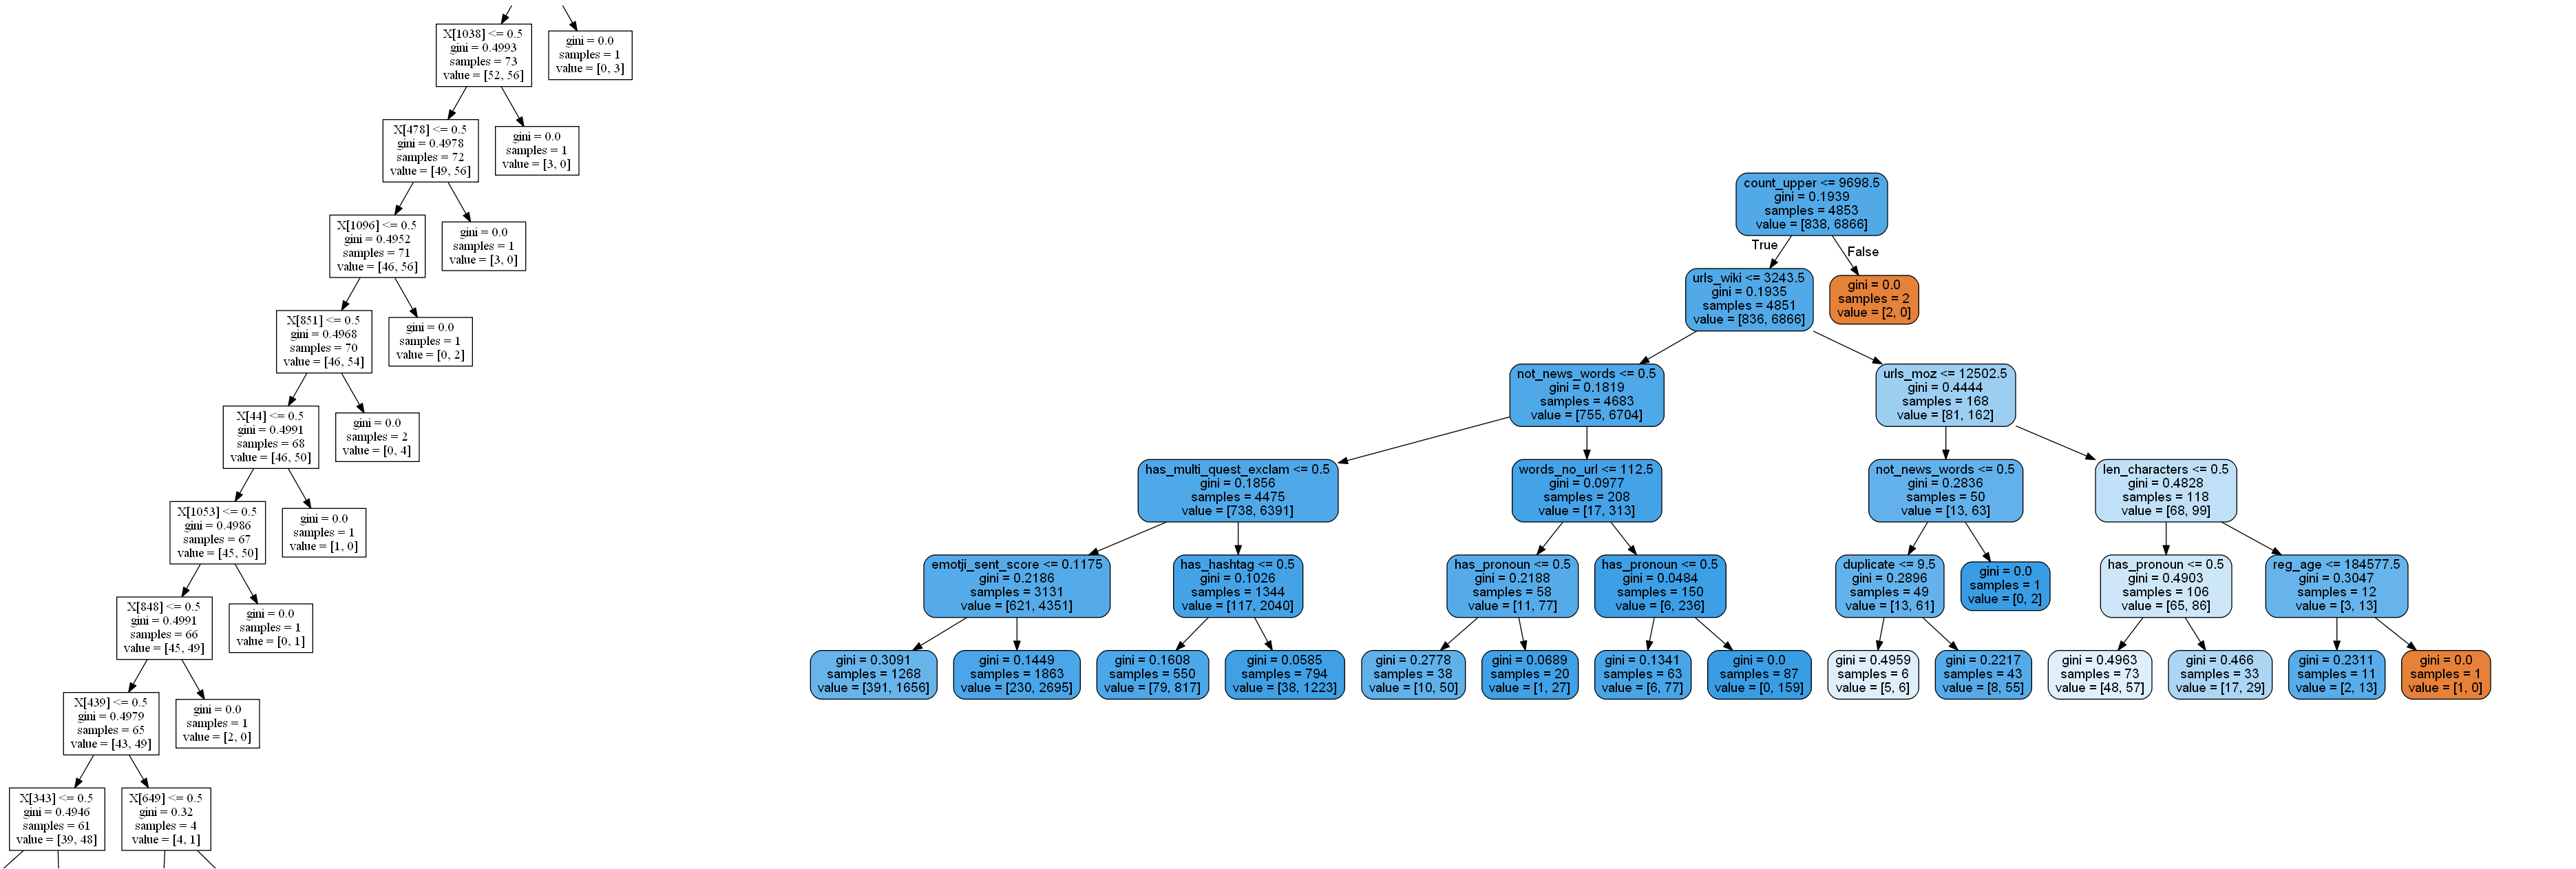
\includegraphics[width=1\textwidth]{decision_tree_sparse_data}
		\captionsetup{width=0.8\textwidth}
		\caption[Decision Tree with Sparse Data]{Decision Tree derived from sparse (Left) and non-sparse (Right) data}
		\label{fig:rand_forest_sparse}
	\end{figure}
		
	\paragraph{ID3 Algorithm} 
		This procedure of Decision Tree induction is known as the ID3 Algorithm (\cite{quinlan1986induction}). More formally, the design functions as follows. We start, as is common in classification problems, with a data training dataset. Each data point (observation) in the set has an assortment of attributes (features) and is assigned to a certain class. At each stage of the tree construction, including the inception stage, a node is created. This node receives as input a group of observations which belong to 2 or more classes. The node than selects a feature of the data and divides the data according to this feature. The feature selection consideration is evaluated with either \hyperref[entropy]{entropy} or the \hyperref[gini]{Gini coefficient}. For each possible value of the previously selected feature, a node is created. If all the samples inside a node belong to a single class, it will not be segmented any further and the node will be denoted as a \textit{leaf}. If, on the other hand, the new node contains data points from different classes, we repeat the process of feature selection and segmentation accordingly. Finally, we want to reach a scenario in which, all leaves of the tree contain observations belonging to a single class each. The contents of such leaves may also referred to as \textit{pure subsets}.
		
	\paragraph{Entropy}
	\label{entropy}
		The priorly mentioned decision rule for feature selection, upon which the data will be split in a given node, can be determined by 2 approaches. Both hold the same principle at their core, this being the amount of certainty gained (\hyperref[info_gain]{Information Gain}) from each split. Hence, the goal is the maximization of certainty, that after a given split, a data point belongs to one distinct class. For example, a feature would be considered a weak feature for splitting, if at a given node it splits the data in a manner where all subsets have relatively similar probabilities of belonging to the different classes. In such an example, no progress was made in the direction of segmenting the data completely. The closer the separation of the data brings us to pure subsets, the higher its ranking as a decision rule at a given node will be. This means, that the lower the entropy values are, the purer the resulting subsets will be.
		
		\par
		One measure which helps quantify the quality of this segmentation rule is \textbf{Entropy}. The calculation of Entropy is demonstrated in equation [\ref{dt_entropy}], with $ S $ being the subset passed to the node as input, $ i \in \{1:c \} $ denoting the different classes and $ p_i $ the percentage of data point corresponding to class $ i $. 
		
		\begin{equation}
			H(S) = \sum_{i=1}^c - p_i \cdot log_2 (p_i)
			\label{dt_entropy}
		\end{equation}
		
	 \paragraph{Gini}
	 \label{gini}
	 	An alternative metric to entropy is the Gini Impurity coefficient. The coefficient denominates the probability of a randomly selected observation to be incorrectly labeled, if the label was set at random according to the actual distribution of labels in the dataset. We compute Gini by summing the probabilities of a given item belonging to a certain class $ i $ multiplied by the probability of misclassification. The Gini impurity is demonstrated in Equation \ref{dt_gini}, with $ i $ denoting a given class, out of $ c $ classes.
	 	
	 \begin{equation}
	 	\begin{aligned}
		 	G(p) &= \sum_{i=1}^c p_i(1-p_i) = \sum_{i=1}^c (p_i-p_i^2) =\sum_{i=1}^c p_i - \sum_{i=1}^c p_i^2 \\  &=  1 - \sum_{i=1}^c p_i^2 = \sum_{i \neq k} p_i p_k
	 	\end{aligned}
		\label{dt_gini}
	 \end{equation}
	 
	 \paragraph{Information Gain}
	 \label{info_gain}	
	 	Entropy allows us to further calculate the Information Gain ($ I_G $) from each split. This gain is calculated in Equation \ref{dt_info_gain}, with $ S $ being the set of input samples, $ v $ a possible value of the attribute $ A $ and $ S_v $ the subset of $ S $ in which the sample attribute $ A $ is equal to $ v $. The gain is therefore, a weighted average of the Entropies, with respect to the prevalence of a given value $ v $ in each subset. Thus, Information Gain also assigns importance to the progress made from a new node. Ergo, a node which classifies few items purely might be outweighed by one which does not split into completely pure subsets, but rather splits correctly a larger amount of items.
	 
			\begin{equation}
			I_G(S,A) = H(S) - \sum_{v \in values(A) } \frac{|S_v|}{S} H(S_v)
			\label{dt_info_gain}
	 \end{equation}
	 
	 \paragraph{Pruning}
		 After the Decision Tree is initially constructed, it undergoes the process of \textit{pruning}. First, the contribution of new knowledge to the classification provided by each branch is calculated. Next, branches with comparably small contributions (have low $ I_G $ values) are removed (\textit{pruned}), in order to simplify the tree. The algorithm is considered efficient and fast since, after pruning the amount of features actually used from a dataset should be relatively small. Ergo, a single sample will be represented through a select few features. Hence, the algorithm is conceptually incompatible with the \hyperref[sec:bag_of_words]{Bag-of-Words} features, due to \hyperref[data_sparsity]{data sparsity}.  In addition, the algorithm is proficient at filtering noise and selecting the best features. Better data attributes are bound to have higher Information Gain values and are therefore more likely to be used in decision nodes.
	
	\paragraph{Random Forest}
		This algorithm builds a boot-strap system on the concept of Decision Trees. The algorithm by \cite{breiman1984classification} builds $ K $ different Decision Trees. Each Decision Tree $ T $ is built using a randomly picked subset $ S $ of the complete dataset. Each such tree is trained using the previously mentioned ID3 algorithm. However each tree does not use all the datasets attributes $ D $ but rather ones selected at random $ d << D $. The trees are not pruned. 
		
		\par
		As a consequence, each of the $ K $ trees is only suitable for a random subset $ S $ of the dataset and examines only a subset $ d $ of attributes. Each tree is not pruned, therefore it classifies its training data perfectly. When classifying novel data, each new observation is classified using all $ K $ trees simultaneously and the most commonly appearing classification decides the class. Therefore, the process implements a voting classification strategy using a \textit{Forest} of Decision Trees. A measure of confidence can also be attached to the classification by counting the percent of all the \textit{trees} in the \textit{Random Forest}, which voted for the resulting class.
 
	
	
